\documentclass{article}
\usepackage{iclr2027_conference,times}
\usepackage[T1]{fontenc}
\usepackage{amsmath,amssymb,booktabs,tabularx,microtype}
\usepackage{hyperref}
\usepackage{url}
\usepackage[section]{placeins}
\newcommand{\TODO}{\texttt{TODO}}
\usepackage{tikz}
\usetikzlibrary{arrows.meta,positioning}
\setlength{\emergencystretch}{2em}
\title{CoSpRo: Concept-Guided\\Relational Pretraining for\\Spurious-Correlation Robustness}
\author{}
\begin{document}
\maketitle
\raggedbottom
\begin{abstract}
Self-supervised representations can encode correlations between an object and
its background that fail outside the training distribution. We introduce
CoSpRo, a method that uses sparse language-aligned concepts to construct
relational supervision for a separate visual encoder. CoSpRo removes selected
concept subspaces from frozen CLIP embeddings and searches for image pairs
whose similarity increases. Residual concept agreement and synthetic null
controls filter these relations into a sparse teacher graph. A ResNet student
combines SimCLR with graph-aware batching and a confidence-weighted relational
loss; the teacher is discarded at inference. Graph construction and student
pretraining require no target or group labels. Under a fixed group-balanced
linear-probe protocol on Waterbirds test, CoSpRo reaches $53.38\pm1.84\%$
average accuracy and $50.64\pm1.97\%$ worst-group accuracy across four seeds,
compared with $51.97\pm2.00\%$ and $46.82\pm3.65\%$ for SimCLR. Matched
controls separate sampling, generic CLIP supervision and concept-projected
relations. Positive test means coexist with mixed seed-wise effects and a
failed earlier validation replication criterion. A separate two-seed
validation screen at SimCLR temperature 0.05 finds that direct SpLiCE
reconstruction transfer improves both metrics over matched SimCLR, raw CLIP
and shuffled targets on both seeds, reversing the conclusion of the earlier
temperature-0.5 screen. These results support useful concept transfer under
specific training conditions, without establishing consistent superiority or
causal removal of background information.
\end{abstract}

\section{Introduction}
An image can contain several predictive factors. In Waterbirds, bird category
correlates with background in the training set. A representation that strongly
encodes this association can fail on birds shown in an uncommon environment.
Worst-group evaluation makes these failures visible even when aggregate accuracy
appears acceptable \citep{sagawa2020groupdro}. Self-supervised pretraining inherits
the correlations present in its unlabeled images. Standard view augmentation
alone does not specify which context changes should preserve object identity.

Our goal is to learn a visual encoder whose downstream predictions remain useful
when object--context associations change, using no target labels or group
annotations during graph construction and representation learning. A frozen
vision-language model supplies semantic structure learned from external data.
SpLiCE exposes this structure as sparse non-negative coordinates associated with
text concepts \citep{bhalla2024splice}. We hypothesize that a concept subspace can
explain why two images appear dissimilar. Removing that subspace may reveal a
useful relation for student training. This hypothesis requires empirical checks:
concepts can also encode object identity and projection can introduce incorrect
neighbours.

CoSpRo constructs a fixed teacher graph from these projected relations.
Each candidate relation is evaluated using geometric gain, concept activation
contrast and agreement in the remaining sparse coordinates. Synthetic nulls
calibrate group selection. The graph determines batch composition and supplies
soft relational targets on the student backbone. At deployment, only the trained
encoder and downstream classifier are required.

Our contribution is a concept-projected relation-discovery method and a
controlled study of its transfer to an independently trained encoder. The graph
exposes which concept removal produced each retained relation. The experimental
design separates this choice of neighbours from graph-aware sampling and generic
CLIP supervision. We report a four-seed validation and held-out comparison,
a matched semantic-graph ablation, and direct prediction of frozen SpLiCE
representations at two contrastive temperatures. These studies distinguish
positive average transfer from seed-wise consistency and graph-mechanism claims.

\section{Related Work}
\paragraph{Concept representations and interventions.}
Concept-based models express predictions through variables that can be examined
and changed. Concept Bottleneck Models first predict a set of annotated concepts
and then use them to predict the target label; editing a concept changes the
downstream prediction \citep{koh2020cbm}. This gives interventions a direct role
in the classifier, but requires a suitable concept set and supervision for its
attributes. CLIP learns a shared image--text representation from large-scale
paired data \citep{radford2021clip}. SpLiCE expresses CLIP embeddings as sparse
non-negative combinations of text-concept directions
\citep{bhalla2024splice}. Its vocabulary provides our intervention coordinates
without concept annotations for the training images. CoSpRo groups these
coordinates and temporarily removes their span from the frozen representation.
The resulting neighbours supervise a separate encoder. Its predictions do not
pass through a concept bottleneck, and the semantic interpretation of a removed
direction does not by itself establish that the direction represents background.

\paragraph{Mitigating spurious correlations.}
Group DRO optimizes the worst loss over annotated training groups and shows the
importance of regularization for worst-group generalization
\citep{sagawa2020groupdro}. Just Train Twice uses errors from an initial
classifier to identify examples for upsampling, reducing the need for training
group annotations while retaining target supervision \citep{liu2021jtt}.
CoBalT discovers object-centric concepts from unlabeled images and uses them to
balance supervised learning across the discovered structure
\citep{arefin2024cobalt}. Its concept discovery is unsupervised, while its final
classifier still uses class labels. DIAL instead removes spurious directions
from vision-language representations through sparse-autoencoder analysis
\citep{yalavarthi2026dial}. This is close to our use of a representation-space
intervention. CoSpRo uses the intervention to discover training relations rather
than to define the deployed representation. We study the encoder learned from
those relations under a fixed supervised linear-probe protocol. Accuracies from
supervised group-robust training or zero-shot VLM evaluation therefore answer
different questions from the matched SSL comparisons reported here.

\paragraph{Self-supervision and relational transfer.}
SimCLR learns from two augmented views of the same image through a contrastive
projection head \citep{chen2020simclr}. The objective does not distinguish
object features from background features when both agree across views.
Learning-speed-aware SSL addresses this problem by sampling examples inversely
to their learning speed \citep{zhu2023lassl}. CoSpRo changes batch composition
using a fixed semantic graph, which makes a sampler-only control necessary.
NNCLR uses nearest neighbours as cross-image positives
\citep{dwibedi2021nnclr}; CoSpRo retains the original within-image positives
and adds a separate relational loss on the backbone. Relational Knowledge
Distillation transfers relationships between examples rather than requiring
teacher and student features to share coordinates \citep{park2019rkd}.
Our KL objective follows this relational approach, but its targets come from
concept-projected neighbourhoods instead of the unmodified teacher geometry.
The matched raw-CLIP graph tests the value of that change under the same
supervision budgets. Direct SpLiCE reconstruction transfer provides a separate
comparison in which the student predicts the teacher's feature coordinates.

\section{Problem Setting}
Let $\mathcal{D}=\{x_i\}_{i=1}^{N}$ be unlabeled training images with stable
sample identifiers. The learned representation is $f_\theta(x)$. A downstream
classifier $w$ predicts target $y$ from frozen features. For evaluation groups
$g=(y,a)$ defined by target and context $a$, we report empirical average accuracy
and worst-group accuracy:
\begin{equation}
 \mathrm{Avg}=\frac{1}{n}\sum_{i=1}^{n}\mathbf{1}\{w(f_\theta(x_i))=y_i\},\qquad
 \mathrm{WGA}=\min_g\frac{1}{n_g}\sum_{i:g_i=g}\mathbf{1}\{w(f_\theta(x_i))=y_i\}.
\end{equation}
Graph discovery and SSL use images and frozen representations. Labels and group
annotations enter downstream probe fitting, balanced probe-subset construction
and post-hoc analysis. The discovery cache rejects annotation fields.
``Label-free'' refers to the graph and SSL stages. It does not describe CLIP's
external image--text pretraining or the supervised evaluation stage. We report
validation development and held-out test results separately. Only the fixed
five-arm, four-seed ordinary-CoSpRo matrix has held-out results; direct-transfer,
semantic-graph and concept-grouping screens remain validation-only.

\section{Method}
\begin{figure}[htbp]
\centering
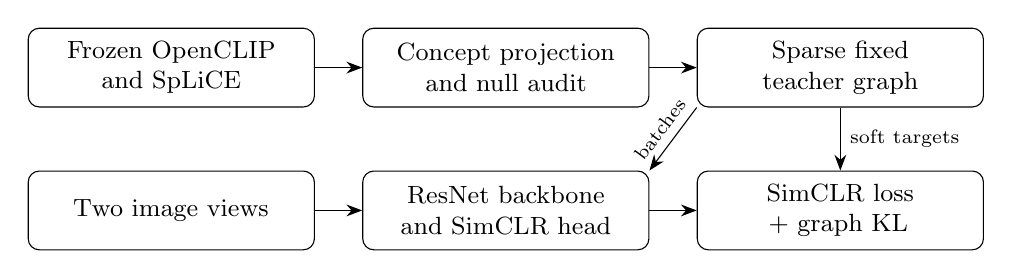
\begin{tikzpicture}[node distance=5mm and 6mm,
 box/.style={draw,rounded corners,align=center,font=\small,minimum height=10mm,text width=34mm},
 >={Stealth[length=2mm]}]
\node[box] (teacher) {Frozen OpenCLIP\\and SpLiCE};
\node[box,right=of teacher] (audit) {Concept projection\\and null audit};
\node[box,right=of audit] (graph) {Sparse fixed\\teacher graph};
\node[box,below=8mm of teacher] (views) {Two image views};
\node[box,right=of views] (student) {ResNet backbone\\and SimCLR head};
\node[box,right=of student] (loss) {SimCLR loss\\+ graph KL};
\draw[->] (teacher)--(audit); \draw[->] (audit)--(graph);
\draw[->] (views)--(student); \draw[->] (student)--(loss);
\draw[->] (graph)--node[right,font=\scriptsize]{soft targets}(loss);
\draw[->] (graph.south west)--node[above,sloped,font=\scriptsize]{batches}(student.north east);
\end{tikzpicture}
\caption{CoSpRo. The frozen branch uses training images to construct the
graph once. Graph construction and student pretraining consume no target or
group annotations. The backbone is evaluated with a supervised linear probe.}
\label{fig:architecture}
\end{figure}
\subsection{Frozen representations and semantic groups}
Frozen OpenCLIP produces unit-normalized image embeddings $z_i$. The fixed SpLiCE centering vector $\mu$
defines centered normalized embeddings
\begin{equation}
 u_i=\operatorname{norm}(z_i-\mu).
\end{equation}
SpLiCE supplies codes $c_i\in\mathbb{R}^{K}_{\geq0}$ and a normalized text dictionary
$D\in\mathbb{R}^{K\times d}$. All feature vectors are columns. The sparse
reconstruction is $D^\top c_i$. The underlying positive sparse regression
minimizes $\|u_i-D^\top c_i\|_2^2+\lambda_1\|c_i\|_1$ over $c_i\geq0$.
Cache rows, vocabulary entries and dictionary directions have explicit alignment.

The ordinary pipeline filters concepts by their occurrence frequency. Lexical
families are joined and additional pairs are joined when text similarity and
coactivation cosine exceed their configured thresholds. Connected components
form flat concept groups. For a group $G$, an SVD of its dictionary directions
provides an orthonormal column basis $Q_G$. The retained singular values satisfy
$\sigma>10^{-6}\max(\sigma_{\max},1)$.
Lexical grouping uses normalized word forms; the additional similarity edges
use the configured text and activation thresholds.

\subsection{Concept projection and relation evidence}
The projection acts on the full centered embedding:
\begin{equation}
 u_i^{-G}=\operatorname{norm}\!\left(u_i-Q_GQ_G^\top u_i\right),
 \label{eq:projection}
\end{equation}
Degenerate projections with norm at most $10^{-12}$ are rejected. Projected
nearest neighbours provide candidate donors. Their gain is
\begin{equation}
 \Delta_{ij}^{G}=\cos(u_i^{-G},u_j^{-G})-\cos(u_i,u_j).
\end{equation}
Group activation is $A_i^G=\sum_{k\in G}c_{ik}$. Candidate edges require a positive
gain above the configured minimum and an activation difference at least as large as the
configured quantile of positive-gain candidates.

With the residual gate enabled, the remaining code coordinates define
\begin{equation}
 R_{ij}^{-G}=\cos(c_i^{-G},c_j^{-G}),\qquad R_{ij}^{-G}\geq\tau_R.
\end{equation}
Zero residual norm receives similarity zero. Disabling the gate sets
$R_{ij}^{-G}=1$ in the evidence and scoring equations. Accepted pair evidence is
\begin{equation}
 e_{ij}^{G}=\Delta_{ij}^{G}\left(\tfrac12+\tfrac12R_{ij}^{-G}\right).
\end{equation}
The group score combines median accepted gain, anchor coverage, mean residual
agreement and the non-negative correlation between activation difference and gain.
The correlation is computed over all positive-gain candidates before the residual
gate; the other three statistics use accepted edges.
A hubness penalty uses destination indegree Gini and maximum indegree:
\begin{equation}
 S(G)=\frac{\operatorname{medianGain}(G)\operatorname{coverage}(G)
 \operatorname{agreement}(G)\operatorname{alignment}(G)}
 {1+\operatorname{Gini}(G)+\operatorname{maxIndegree}(G)/N}.
\end{equation}

\subsection{Null calibration and sparse teacher graph}
Equal-rank random subspaces and shuffled group activations produce null scores.
Random bases are obtained from Gaussian directions and induce new projected
neighbours while retaining the original group's activation vector and residual
coordinate mask. Activation shuffling permutes that vector across images while
retaining the group's projection geometry and residual agreement. Each control
is scored with the same relation-selection rule as the candidate group.
Their pooled configured quantile is $T_G$. A group passes when it has sufficient
coverage and $S(G)>T_G$. Its evidence is scaled by
\begin{equation}
 r_G=\min\!\left(1,\frac{\max(0,S(G)-T_G)}{\max(|S(G)|,\epsilon)}\right),
 \qquad \tilde e_{ij}^{G}=r_Ge_{ij}^{G}.
\end{equation}
The configured group cap keeps the largest null-excess scores after the audit.
Duplicate directed edges retain
the strongest evidence. Outgoing top-$k$ pruning and an absolute destination
indegree cap yield a sparse graph. Supported rows define
\begin{equation}
 p_T(j\mid i)=\frac{\tilde e_{ij}}{\sum_k\tilde e_{ik}},\qquad
 q_i=\operatorname{clip}_{[0,1]}\max_j\tilde e_{ij}.
\end{equation}
The row probabilities specify relative donor preferences and $q_i$ carries
absolute evidence strength. Unsupported anchors have zero relational contribution.
The trainer supports an empty-graph SimCLR fallback. The matched control runner
requires a nonempty graph to preserve the intended experimental contrasts.

\subsection{Graph-aware student training}
The sampler visits each image exactly once per SSL epoch and places a sampled
available teacher neighbour in the same batch when possible. A ResNet backbone
produces two augmented-view features $h_i^{(1)}$ and $h_i^{(2)}$. The relational
representation is
\begin{equation}
 s_i=\operatorname{norm}\!\left[\operatorname{norm}(h_i^{(1)})+
 \operatorname{norm}(h_i^{(2)})\right].
\end{equation}
A softmax over backbone similarities defines the student distribution
\begin{equation}
 p_S^B(j\mid i)=\frac{\exp(s_i^\top s_j/\tau_S)}
 {\sum_{k\in B:k\ne i}\exp(s_i^\top s_k/\tau_S)},\quad j\ne i.
\end{equation} Occurrences of the anchor sample are masked. Restricting
$p_T$ to batch donors and renormalizing gives $p_T^B$. The objective is
\begin{align}
 \mathcal{L}_{\mathrm{graph}}&=\frac{1}{|B_S|}\sum_{i\in B_S}q_i
 D_{\mathrm{KL}}\!\left(p_T^B(\cdot\mid i)\,\|\,p_S^B(\cdot\mid i)\right),\\
 \mathcal{L}(t)&=\mathcal{L}_{\mathrm{SimCLR}}+
 \lambda(t)\mathcal{L}_{\mathrm{graph}}.
\end{align}
Here $B_S$ contains anchors with an in-batch teacher donor; an empty $B_S$
contributes zero loss. SimCLR uses a separate projection head $g_\phi$.
Let $v_a=\operatorname{norm}(g_\phi(h_a))$ index the $2|B|$ augmented views
and let $a^+$ denote the other view of the same image. Then
\begin{equation}
 \mathcal{L}_{\mathrm{SimCLR}}=-\frac{\tau_C}{0.07}\frac{1}{2|B|}\sum_{a=1}^{2|B|}
 \log\frac{\exp(v_a^\top v_{a^+}/\tau_C)}
 {\sum_{b\ne a}\exp(v_a^\top v_b/\tau_C)}.
\end{equation}
The prefactor $\tau_C/0.07$ follows the implemented loss normalization and
fixes the scale relative to the graph term. Teacher neighbours affect batch
composition and backbone supervision; the
positive pair in this contrastive objective remains the two views of one image.
KL starts after epoch 10 and warms up over ten epochs to its maximum weight.
We use $\lambda_{\max}=0.5$ for the main comparison and examine 0.2 and 2
in the weight study. The weight remains constant after warm-up through epoch 500.

\section{Experimental Protocol}
\paragraph{Data and representations.}
Waterbirds contains 4,795 training images with group counts 3,498, 184, 56 and
1,057 in $(y,a)$ order 00, 01, 10 and 11. Validation contains 1,199 images with
counts 467, 466, 133 and 133. The frozen teacher is OpenCLIP ViT-B/32 with the
\texttt{laion2b\_s34b\_b79k} checkpoint. The dictionary uses the complete cleaned
Open Images V7 vocabulary and sparse regression weight 0.25. The corresponding
signal artifact has 20,931 concept coordinates. The image mean is the frozen
SpLiCE centering vector stored in the cache. Every downstream comparison uses
the same train/validation split.

\paragraph{Student optimization.}
The student is a randomly initialized ResNet-18 with the ImageNet-style stem
(\texttt{resnet18\_large}). Training uses 500 SSL epochs, batch size 128 and SGD
with learning rate 0.01, momentum 0.9 and weight decay $10^{-4}$. Learning rate
is multiplied by 0.1 at epochs 350, 400 and 450. SimCLR temperature is 0.05;
relational temperature is 0.25. Standard views use random resized crops with
minimum scale 0.2, horizontal flips, color jitter and grayscale conversion.
The main study has student seeds 1--4 with one locked graph seed 0.
Weights 0.2 and 0.5 were first screened on seeds 1 and 2. The selected weight
0.5 was then evaluated on seeds 3 and 4 using the same frozen graphs. We report
both the pooled estimates and the replication subset; the pooled estimates
remain conditional on validation-based selection.

\paragraph{Linear evaluation.}
Every 25 SSL epochs, a frozen-feature logistic probe is fitted on the
\texttt{ds\_train} subset containing 56 examples per group (224 total).
The subset uses training-group annotations. Training statistics standardize
features. Full-batch float64 L-BFGS minimizes mean cross-entropy with L2
coefficient 0.001 on classifier weights. Convergence requires ten consecutive
external optimization epochs with maximum absolute objective gradient below
$10^{-6}$. Each external step allows up to 20 inner iterations with a safety
limit of 200 external epochs. Reported metrics average the final ten converged
probe optimization epochs. All student comparisons use the representation at SSL
epoch 500. These ten optimization epochs are not independent experimental
replicates. Standard deviations below are sample deviations across student seeds.

\paragraph{Controls.}
SimCLR uses standard batches and no graph loss. CoSpRo sampler-only uses graph-aware
batches with KL weight zero. Raw-CLIP sampler-only provides the corresponding
control for the raw teacher. The raw-CLIP teacher uses centered-CLIP neighbours
with CoSpRo's supported anchors, outgoing row budgets, row weight profiles and
anchor confidence. Both graphs obey the same maximum indegree. Each teacher
induces its own batches, so the KL comparison must also be interpreted alongside
the two sampler-only arms.

\paragraph{Reproducibility and held-out evaluation.}
Matched seeds share initialization; teacher loading and periodic probes are
isolated from the training RNG. The evidence archive contains configurations,
graph identities and all 680 periodic probe records from the 34 graph-study
runs. Every epoch-500 probe satisfies the convergence criterion. Historical
probe views depend partly on the run seed, so the reported deviation describes
the complete training-and-evaluation run. Some older saved feature tensors
require reconstruction of the seeded loader order because they lack explicit
sample IDs. Appendix~\ref{app:provenance} records these provenance limits.
Held-out evaluation uses the selected configuration, the same training subset
for probe fitting and the epoch-500 encoder. The completed 20-model matrix is
reported below and in Appendix~\ref{app:test}. Its saved lock excludes the
additional screening branches and prohibits test-driven tuning. Checkpoint
hashes and final metrics were verified; remaining source and probe-provenance
limitations are disclosed in Appendix~\ref{app:provenance}.

\section{Results}
\subsection{Matched Waterbirds comparison}
\begin{table}[htbp]
\centering
\caption{Waterbirds validation at SSL epoch 500, seeds 1--4. Both KL arms use
$\lambda_{\max}=0.5$. Values are percentages (mean $\pm$ sample standard
deviation). The four-seed estimate includes the development seeds 1 and 2.}
\begin{tabular}{lrr}
\toprule
Method & Avg. & WGA \\
\midrule
SimCLR & $52.11 \pm 1.37$ & $45.54 \pm 1.71$ \\
CoSpRo sampler only & $52.46 \pm 3.60$ & $47.39 \pm 4.06$ \\
Raw CLIP sampler only & $50.96 \pm 2.36$ & $44.27 \pm 2.95$ \\
Raw CLIP + KL & $51.54 \pm 2.07$ & $46.97 \pm 2.83$ \\
CoSpRo + KL & $53.46 \pm 3.05$ & $50.00 \pm 3.23$ \\
\bottomrule
\end{tabular}
\label{tab:main}
\end{table}

CoSpRo improves mean WGA by 4.46 percentage points relative to SimCLR and
3.02 points relative to matched raw-CLIP supervision (Table~\ref{tab:main}).
The corresponding average-accuracy differences are +1.36 and +1.92 points.
Graph-aware sampling accounts for part of the change: the CoSpRo sampler-only
arm reaches 47.39\% WGA, compared with 45.54\% for ordinary SimCLR.

The replication subset gives a weaker result than the initial screen.
On seeds 3 and 4, CoSpRo changes mean Avg./WGA by $-0.71/+2.22$ points
relative to SimCLR and $-1.50/+0.18$ relative to its own sampler.
The prespecified replication criterion required positive mean differences in
both metrics against SimCLR, the CoSpRo sampler and all three raw-CLIP KL
weights on these two seeds, together with pooled gains of at least 1 point
Avg. and 2 points WGA over SimCLR. It is not met. The pooled average therefore
does not establish consistent joint improvement over the controls.

The effect is not confined to the final probe. Across epochs 400--500,
seed-3 CoSpRo averages 49.51/45.58\% Avg./WGA versus 52.78/47.28\% for
SimCLR. On seed 4, the corresponding values are 55.46/53.10\% and
53.56/47.52\%. These correlated late-epoch measurements describe stability;
the primary endpoint remains epoch 500. Appendix~\ref{app:seedresults}
reports each seed and all four groups.

\subsection{Held-out Waterbirds comparison}
\begin{table}[htbp]
\centering\small
\setlength{\tabcolsep}{4pt}
\caption{Waterbirds held-out test at SSL epoch 500. Both KL arms use weight 0.5; mean $\pm$ sample SD over seeds 1--4. These are separate from validation in Table~\ref{tab:main}.}
\begin{tabular}{lrr}
\toprule
Method & Avg. & WGA \\
\midrule
SimCLR & $51.97 \pm 2.00$ & $46.82 \pm 3.65$ \\
CoSpRo sampler & $51.95 \pm 3.32$ & $46.83 \pm 1.29$ \\
Raw CLIP sampler & $50.86 \pm 2.61$ & $45.88 \pm 5.98$ \\
Raw CLIP + KL & $52.64 \pm 2.39$ & $48.48 \pm 3.44$ \\
CoSpRo + KL & $53.38 \pm 1.84$ & $50.64 \pm 1.97$ \\
\bottomrule
\end{tabular}
\label{tab:testmain}
\end{table}

CoSpRo has the highest mean Avg. and WGA in the fixed test matrix
(Table~\ref{tab:testmain}). Relative to SimCLR its gains are $+1.41/+3.82$
points Avg./WGA; relative to raw-CLIP KL they are $+0.74/+2.16$ points.
Against its own sampler the differences are $+1.43/+3.81$ points, with
positive WGA differences on all four seeds. Joint gains over SimCLR occur
on three seeds; seed 3 changes by $-1.19/-1.02$ points. Joint gains over
raw-CLIP KL occur on only two seeds.

Descriptive paired-$t$ 95\% intervals for WGA are $[-2.85,10.50]$ points
against SimCLR, $[-1.06,5.38]$ against raw-CLIP KL and $[1.67,5.95]$
against the CoSpRo sampler. They use four pairs without multiplicity
correction and do not remove development-seed selection effects. Positive
test means support transfer under the fixed protocol, but do not establish
consistent superiority or override the failed validation replication gate.
All test seeds, group accuracies and paired contrasts appear in
Appendix~\ref{app:test}.

\subsection{Exploratory KL-weight screen}
\begin{table}[t]
\centering
\caption{Two-seed weight screen on Waterbirds validation. Each mean uses seeds
1 and 2. Weight 2 is the original reference setting.
The same validation set informed this exploratory screen.}
\begin{tabular}{rlrrrr}
\toprule
$\lambda_{\max}$ & Teacher & Avg. s1 & Avg. s2 & Mean Avg. & Mean WGA \\
\midrule
0.2 & Raw CLIP & 53.71 & 49.96 & 51.83 & 48.42 \\
0.2 & CoSpRo & 51.21 & 49.37 & 50.29 & 44.65 \\
0.5 & Raw CLIP & 50.38 & 49.46 & 49.92 & 45.45 \\
0.5 & CoSpRo & 55.80 & 53.29 & 54.55 & 50.80 \\
2 & Raw CLIP & 53.13 & 51.79 & 52.46 & 46.79 \\
2 & CoSpRo & 51.38 & 51.96 & 51.67 & 48.07 \\
\bottomrule
\end{tabular}
\label{tab:weights}
\end{table}

The initial screen favors weight 0.5 over 0.2 and 2
(Table~\ref{tab:weights}). Replication extends the 0.5 comparison to four
seeds. Relative to weight 2, CoSpRo at 0.5 improves Avg. and WGA on every
seed; the mean differences are +2.25 and +4.08 points. This consistency across
weights is stronger than the evidence for superiority to SimCLR. Raw-CLIP KL
at weights 0.2, 0.5 and 2 reaches four-seed WGA of 47.09\%, 46.97\% and
45.10\%, respectively. Weight 0.5 is a validation-selected setting, not an
independently confirmed optimum.

\subsection{What the frozen diagnostics establish}
Frozen SpLiCE reconstruction retains useful supervised signal (77.98\%
Avg., 72.75\% WGA), but this is a teacher diagnostic rather than a matched
student result. The fixed graph contains 12 selected concept groups and
12,239 edges. For training waterbirds on land, wrong-target edges carry
45.76\% of CoSpRo's confidence-weighted mass versus 39.73\% for raw CLIP.
Thus, semantic projection can introduce incorrect relations despite positive
average downstream effects. Appendix~\ref{app:diagnostics} reports the full
frozen-feature comparison, source-group edge composition and reconstruction
and sampler-exposure diagnostics.

\subsection{Direct transfer of frozen representations}
We compare relational transfer with direct prediction of a frozen target.
A separate head $g_\psi$ predicts a unit-normalized target $t_i$ from each
student view:
\begin{equation}
 \mathcal{L}_{\mathrm{transfer}}=
 \frac{1}{2|B_V|}\sum_{i\in B_V}\sum_{v=1}^{2}
 \left[1-\cos\!\left(g_\psi(f_\theta(x_i^{(v)})),t_i\right)\right].
\end{equation}
Targets are centered raw-CLIP embeddings, normalized SpLiCE reconstructions
or a fixed derangement of the reconstructions. $B_V$ contains valid target
rows. The training objective is
$\mathcal{L}_{\mathrm{SimCLR}}+\alpha(t)\mathcal{L}_{\mathrm{transfer}}$;
the matched SimCLR arm retains the head with $\alpha=0$.
All four arms use ordinary batches, seeds 1 and 3, 500 epochs and maximum
transfer weight 0.1 after the same delay and warm-up. The initial screen used
SimCLR temperature 0.5. A subsequent eight-run screen fixes it to 0.05,
retaining the target definitions, head, weight, optimization schedule and
augmentation recipe. The subsequent runs also record AMP-scaled gradient
diagnostics. Each comparison uses its own matched direct baseline; the two
temperatures and the graph study are not pooled.



SpLiCE reconstruction improves both metrics on seed 1 and reduces both on
seed 3 (Table~\ref{tab:direct}). Its mean differences from matched SimCLR
are $-1.92$ points Avg. and $-6.05$ points WGA. It does not meet the
prespecified screen criterion of positive Avg./WGA differences on both seeds,
mean gains of at least 1/2 points over SimCLR and positive mean differences
in both metrics over raw and shuffled targets. Removing the sparse-graph
transfer step is therefore insufficient under this direct-transfer recipe.

\begin{table}[htbp]
\centering\small
\setlength{\tabcolsep}{4pt}
\caption{Corrected direct transfer at SimCLR temperature 0.05. Validation percentages at SSL epoch 500, reported as Avg./WGA. Separate from the historical temperature-0.5 screen.}
\begin{tabular}{lrrr}
\toprule
Target & Seed 1 & Seed 3 & Mean \\
\midrule
Matched SimCLR & 50.29 / 44.54 & 52.63 / 47.32 & 51.46 / 45.93 \\
Raw CLIP & 52.96 / 45.86 & 52.88 / 49.62 & 52.92 / 47.74 \\
SpLiCE reconstruction & 54.71 / 50.75 & 53.54 / 50.11 & 54.13 / 50.43 \\
Shuffled reconstruction & 51.96 / 46.68 & 51.54 / 46.47 & 51.75 / 46.57 \\
\bottomrule
\end{tabular}
\label{tab:direct005}
\end{table}

At temperature 0.05, reconstruction improves both metrics on both seeds
against all three matched controls (Table~\ref{tab:direct005}). Mean gains
are $+2.67/+4.50$ points Avg./WGA over SimCLR, $+1.21/+2.68$ over raw CLIP
and $+2.38/+3.85$ over shuffled reconstruction. Its mean $\pm$ sample SD
is $54.13\pm0.83\%$ Avg. and $50.43\pm0.45\%$ WGA. The two-seed screen
criterion is met. The raw-CLIP contrast supports a preliminary benefit from
the SpLiCE target representation, while the shuffled contrast supports
image-specific correspondence. Both seeds were reused from development;
this is a positive validation screen, not held-out confirmation of direct
transfer or evidence for the CoSpRo projection mechanism.

The corrected histories record finite nonzero encoder transfer gradients.
At epoch 500, across two reconstruction seeds and four diagnostic batches
each, the mean transfer-to-SimCLR gradient-norm ratio is 0.00857; the
corresponding values are 0.00719 for raw targets and 0.000842 for shuffled
targets. Reconstruction's mean gradient cosine is 0.0102. These limited
batch diagnostics show that the transfer signal reaches the encoder; they
do not establish causal mediation. A separate FP32-equivalence and
unchanged-update verification report remains unavailable in the local archive.


\subsection{Semantic relations and concept grouping}
The completed semantic-graph control uses nearest neighbours of the normalized
SpLiCE reconstruction while preserving CoSpRo's supported anchors, row budgets,
weight profiles and confidence. It tests whether intervention-derived relations
add value beyond ordinary SpLiCE similarity. Because neighbour identity also
affects batches, the comparison concerns the complete graph-transfer pipeline.
Both graphs have 12,239 edges, 4,582 supported anchors and maximum indegree 10.
The saved preflight verifies sample alignment; a complete archived comparison
of row weights, confidence and edge overlap remains to be packaged.

\begin{table}[htbp]
\centering\small
\setlength{\tabcolsep}{4pt}
\caption{Matched graph-ablation validation at epoch 500, weight 0.5 and SimCLR temperature 0.05. Entries are Avg./WGA percentages.}
\begin{tabular}{lrrr}
\toprule
Teacher & Seed 1 & Seed 3 & Mean \\
\midrule
CoSpRo & 55.80 / 51.61 & 49.21 / 45.49 & 52.50 / 48.55 \\
SpLiCE similarity graph & 54.05 / 44.36 & 49.79 / 43.90 & 51.92 / 44.13 \\
\bottomrule
\end{tabular}
\label{tab:semantic}
\end{table}

CoSpRo gains $+0.58/+4.42$ points Avg./WGA on average
(Table~\ref{tab:semantic}). WGA differences are positive on both seeds
($+7.25$ and $+1.60$), but Avg. differences change sign ($+1.75$ and
$-0.58$). This supports a WGA benefit of intervention-derived relations
under these matched budgets, with uncertain average-accuracy benefit.


A separate exploratory concept-grouping screen constructs a new
intervention-based graph, rather than replacing intervention neighbours by
reconstruction neighbours. It has 12,281 edges and 4,593 supported anchors.
Its Avg./WGA is $50.67\pm0.06/46.95\pm1.59\%$, compared with
$52.50\pm4.66/48.55\pm4.32\%$ for its ordinary-CoSpRo baseline.
Mean differences are $-1.83/-1.60$ points: seed 1 loses $5.09/5.78$ points
and seed 3 gains $1.42/2.58$. These mixed outcomes do not support replacing
the original grouping. Its baseline repeats the semantic-ablation CoSpRo
values on the same seeds; it does not add independent replication evidence.

Randomized-graph SSL remains untested. Frozen construction nulls and shuffled
direct targets do not establish downstream superiority to an arbitrary graph.
This bounds the semantic interpretation of the graph results without making
another training series a prerequisite for reporting the present findings.

The planned qualitative analysis uses actual selected concepts and retained edges.
The most represented groups include Bamboo, Great grey owl and Tawny owl;
each is a singleton in the selected graph. The panel selection fixes groups
by attributed edge count and samples high- and low-gain pairs before inspecting
images. Each panel pairs raw and projected similarities with retained/rejected
status. The image panels remain \TODO{}; concept names alone cannot verify
what visual difference a projection removes.

\section{Limitations}
The experiments cover Waterbirds and one frozen graph seed. Validation was
reused for development, and four student seeds leave substantial uncertainty
about the average effect. The 224-example group-balanced probe uses labels and
group annotations, so label-free pretraining does not make the full evaluation
pipeline unsupervised. The results concern this probe regime and do not estimate
performance under a large fully supervised training budget. The ordinary
five-arm test matrix is complete, but it reuses the development seeds and
does not turn the failed validation replication criterion into a success.
The corrected direct and graph/grouping screens use only two seeds and have
no separate held-out evaluation. Their results must not be used to retune
the already evaluated core test protocol.

Concept names do not uniquely identify causal factors. A direction can contain
both object and background information, and subspace projection does not
generate a counterfactual image. Null calibration compares operational scores;
it does not establish causal identification or control a multiple-testing
false-discovery rate. The wrong-target relations in the graph show why an
increase in cosine similarity is not sufficient evidence of a useful training
pair. Background remains linearly predictable: on test the background probe
reaches 91.72\% for CoSpRo, 91.35\% for SimCLR and 91.42\% for raw-CLIP KL.
Improved WGA therefore does not imply removal of background information,
and the per-group results include losses as well as gains.

The method depends on the frozen encoder, its external pretraining data and the
coverage of the text vocabulary. Sparse reconstruction also discards some CLIP
information. Graph construction adds a frozen preprocessing cost, while each
student uses the same 500-epoch budget as its controls. The teacher is not used
at inference. The reversal between the two direct-transfer temperatures
shows that the result depends on the training recipe; it does not establish
a universally preferable distillation objective. The source snapshot and
probe-identity documentation for the cluster executions remain incomplete,
despite verified retained-model hashes and complete endpoint metrics.

\begin{samepage}
\section{Conclusion}
CoSpRo uses concept-subspace projections to discover relations for
self-supervised pretraining. Its fixed teacher graph supplies a training signal
to a separate encoder without target or group labels during discovery or SSL.
The four-seed Waterbirds comparison gives positive average validation and
held-out effects at weight 0.5: test gains over SimCLR are 1.41 points Avg.
and 3.82 points WGA. Mixed seeds, wide intervals and the failed validation
replication criterion prevent a claim of consistent superiority. The
semantic-graph comparison supports WGA gains from intervention-derived
relations, while some retained relations connect different target classes.
Separately, direct SpLiCE transfer at temperature 0.05 improves both metrics
over SimCLR, raw CLIP and shuffled targets on both validation seeds, unlike
the earlier temperature-0.5 screen. Concept representations can thus provide
useful student supervision under this protocol, while causal background
removal and broader generalization remain unestablished.

\end{samepage}

\begingroup
\footnotesize
\setlength{\bibsep}{4pt plus 1pt}
\begin{thebibliography}{99}
\bibitem[Arefin et~al.(2024)]{arefin2024cobalt}
M.~R.~Arefin, Y.~Zhang, A.~Baratin, F.~Locatello, I.~Rish, D.~Liu and K.~Kawaguchi.
Unsupervised Concept Discovery Mitigates Spurious Correlations.
\emph{ICML}, pp.~1672--1688, 2024.
\url{https://proceedings.mlr.press/v235/arefin24a.html}.
\bibitem[Bhalla et~al.(2024)]{bhalla2024splice}
U.~Bhalla, A.~Oesterling, S.~Srinivas, F.~P.~Calmon and H.~Lakkaraju.
Interpreting CLIP with Sparse Linear Concept Embeddings (SpLiCE).
\emph{NeurIPS}, 2024. \url{https://arxiv.org/abs/2402.10376}.
\bibitem[Chen et~al.(2020)]{chen2020simclr}
T.~Chen, S.~Kornblith, M.~Norouzi and G.~Hinton.
A Simple Framework for Contrastive Learning of Visual Representations.
\emph{ICML}, pp.~1597--1607, 2020.
\url{https://proceedings.mlr.press/v119/chen20j.html}.
\bibitem[Dwibedi et~al.(2021)]{dwibedi2021nnclr}
D.~Dwibedi, Y.~Aytar, J.~Tompson, P.~Sermanet and A.~Zisserman.
With a Little Help From My Friends: Nearest-Neighbor Contrastive Learning
of Visual Representations. \emph{ICCV}, pp.~9588--9597, 2021.
\url{https://arxiv.org/abs/2104.14548}.
\bibitem[Koh et~al.(2020)]{koh2020cbm}
P.~W.~Koh, T.~Nguyen, Y.~S.~Tang, S.~Mussmann, E.~Pierson, B.~Kim and P.~Liang.
Concept Bottleneck Models. \emph{ICML}, pp.~5338--5348, 2020.
\url{https://proceedings.mlr.press/v119/koh20a.html}.
\bibitem[Liu et~al.(2021)]{liu2021jtt}
E.~Z.~Liu, B.~Haghgoo, A.~S.~Chen, A.~Raghunathan, P.~W.~Koh,
S.~Sagawa, P.~Liang and C.~Finn.
Just Train Twice: Improving Group Robustness without Training Group Information.
\emph{ICML}, pp.~6781--6792, 2021.
\url{https://proceedings.mlr.press/v139/liu21f.html}.
\bibitem[Park et~al.(2019)]{park2019rkd}
W.~Park, D.~Kim, Y.~Lu and M.~Cho.
Relational Knowledge Distillation. \emph{CVPR}, pp.~3967--3976, 2019.
\url{https://arxiv.org/abs/1904.05068}.
\bibitem[Radford et~al.(2021)]{radford2021clip}
A.~Radford et~al.
Learning Transferable Visual Models From Natural Language Supervision.
\emph{ICML}, pp.~8748--8763, 2021.
\url{https://proceedings.mlr.press/v139/radford21a.html}.
\bibitem[Sagawa et~al.(2020)]{sagawa2020groupdro}
S.~Sagawa, P.~W.~Koh, T.~B.~Hashimoto and P.~Liang.
Distributionally Robust Neural Networks for Group Shifts: On the Importance
of Regularization for Worst-Case Generalization.
\emph{ICLR}, 2020. \url{https://arxiv.org/abs/1911.08731}.
\bibitem[Wang et~al.(2024)]{wang2024sclip}
F.~Wang, J.~Mei and A.~Yuille.
SCLIP: Rethinking Self-Attention for Dense Vision-Language Inference.
\emph{ECCV}, 2024. \url{https://arxiv.org/abs/2312.01597}.
\bibitem[Yalavarthi et~al.(2026)]{yalavarthi2026dial}
B.~C.~Yalavarthi, N.~Ratha and V.~Govindaraju.
Label-Free Mitigation of Spurious Correlations in VLMs using Sparse Autoencoders.
\emph{ICLR}, 2026.
\href{https://proceedings.iclr.cc/paper_files/paper/2026/hash/359242d225d2fba218a85e147803f8b7-Abstract-Conference.html}{ICLR 2026 proceedings}.
\bibitem[Zhu et~al.(2023)]{zhu2023lassl}
W.~Zhu, S.~Liu, C.~Fernandez-Granda and N.~Razavian.
Making Self-supervised Learning Robust to Spurious Correlation via
Learning-speed Aware Sampling. \emph{arXiv:2311.16361}, 2023.
\url{https://arxiv.org/abs/2311.16361}.
\end{thebibliography}
\endgroup

\clearpage
\appendix
\section{Frozen Audit Configuration}
\begin{table}[ht]
\centering
\begin{tabularx}{\linewidth}{lX}
\toprule
Component & Completed-control setting \\
\midrule
Concept frequency & $[0.01,0.95]$ \\
Grouping & Text cosine 0.80; coactivation cosine 0.35; minimum size 1 \\
Projected neighbours & 20 per image \\
Residual code cosine & At least 0.25 \\
Activation contrast & Positive-gain difference quantile 0.75 \\
Minimum gain / coverage & $10^{-4}$ / 0.01 \\
Null calibration & 32 trials per family; pooled quantile 0.95 \\
Group cap & 12 after the full audit \\
Teacher graph & Up to 3 outgoing edges; maximum indegree 10 \\
Graph seed & 0 shared across student seeds \\
Spatial and CoBalT evidence & Disabled \\
\bottomrule
\end{tabularx}
\end{table}

\section{Per-Seed and Per-Group Results}
\label{app:seedresults}
\begin{table}[htbp]
\centering\small
\setlength{\tabcolsep}{4pt}
\caption{Waterbirds validation at epoch 500; KL weight 0.5. Groups are
$(y,a)$ in order 00, 01, 10, 11. Seeds 1 and 2 informed weight selection;
seeds 3 and 4 form the replication subset. Values are percentages.}
\begin{tabular}{lrrrrrrr}
\toprule
Method & Seed & Avg. & WGA & 00 & 01 & 10 & 11 \\
\midrule
SimCLR & 1 & 50.29 & 44.54 & 44.54 & 50.00 & 54.89 & 66.92 \\
SimCLR & 2 & 51.96 & 43.68 & 43.68 & 58.37 & 52.63 & 57.89 \\
SimCLR & 3 & 52.63 & 47.32 & 47.32 & 56.22 & 51.88 & 59.40 \\
SimCLR & 4 & 53.54 & 46.62 & 53.75 & 50.43 & 46.62 & 70.68 \\
\addlinespace
CoSpRo sampler & 1 & 49.87 & 43.25 & 43.25 & 50.00 & 57.89 & 64.66 \\
CoSpRo sampler & 2 & 52.21 & 48.28 & 50.32 & 48.28 & 57.14 & 67.67 \\
CoSpRo sampler & 3 & 50.13 & 45.40 & 45.40 & 48.50 & 57.89 & 64.66 \\
CoSpRo sampler & 4 & 57.63 & 52.63 & 59.31 & 54.72 & 52.63 & 66.92 \\
\addlinespace
Raw CLIP sampler & 1 & 54.05 & 46.25 & 46.25 & 59.44 & 57.14 & 59.40 \\
Raw CLIP sampler & 2 & 48.46 & 44.42 & 45.82 & 44.42 & 56.39 & 63.91 \\
Raw CLIP sampler & 3 & 50.04 & 40.04 & 40.04 & 52.58 & 60.90 & 65.41 \\
Raw CLIP sampler & 4 & 51.29 & 46.35 & 51.39 & 46.35 & 56.39 & 63.16 \\
\addlinespace
Raw CLIP + KL & 1 & 50.38 & 44.33 & 44.33 & 54.51 & 54.89 & 52.63 \\
Raw CLIP + KL & 2 & 49.46 & 46.57 & 47.11 & 46.57 & 53.38 & 63.91 \\
Raw CLIP + KL & 3 & 52.21 & 46.04 & 46.04 & 51.07 & 65.41 & 64.66 \\
Raw CLIP + KL & 4 & 54.13 & 50.96 & 50.96 & 53.86 & 59.40 & 60.90 \\
\addlinespace
CoSpRo + KL & 1 & 55.80 & 51.61 & 51.61 & 56.22 & 58.65 & 66.17 \\
CoSpRo + KL & 2 & 53.29 & 50.00 & 53.32 & 50.00 & 52.63 & 65.41 \\
CoSpRo + KL & 3 & 49.21 & 45.49 & 46.04 & 45.49 & 60.15 & 62.41 \\
CoSpRo + KL & 4 & 55.55 & 52.89 & 52.89 & 57.30 & 54.89 & 59.40 \\
\addlinespace
\bottomrule
\end{tabular}
\end{table}

\begin{table}[htbp]
\centering\small
\caption{Paired CoSpRo differences in percentage points at epoch 500.
CoSpRo and raw-CLIP KL use weight 0.5.}
\begin{tabular}{rrrrrrr}
\toprule
& \multicolumn{2}{c}{vs. SimCLR} & \multicolumn{2}{c}{vs. own sampler} & \multicolumn{2}{c}{vs. raw CLIP + KL} \\
Seed & $\Delta$Avg. & $\Delta$WGA & $\Delta$Avg. & $\Delta$WGA & $\Delta$Avg. & $\Delta$WGA \\
\midrule
1 & +5.50 & +7.07 & +5.92 & +8.35 & +5.42 & +7.28 \\
2 & +1.33 & +6.32 & +1.08 & +1.72 & +3.84 & +3.43 \\
3 & -3.42 & -1.83 & -0.92 & +0.10 & -3.00 & -0.54 \\
4 & +2.00 & +6.27 & -2.09 & +0.26 & +1.42 & +1.93 \\
\midrule
Mean & +1.36 & +4.46 & +1.00 & +2.61 & +1.92 & +3.02 \\
\bottomrule
\end{tabular}
\end{table}

Across four seeds, a descriptive paired-$t$ 95\% interval for the difference
from SimCLR is $[-4.49,7.20]$ points Avg. and $[-2.24,11.15]$ points WGA.
These intervals do not account for repeated use of validation in development.

\section{Evidence Provenance}
\label{app:provenance}
The accompanying \texttt{paper\_results.json} preserves the historical
validation study and adds the completed test, corrected-direct, graph-ablation
and grouping results as separate blocks. The historical graph/weight study
contains 34 runs and 680 periodic probes; the prior audit verified 755 source
digests. The completion archive adds 20 core executions with retained models,
400 validation probe records and 20 test JSON/tensor pairs. All 20 checkpoint
SHA-256 digests match the saved final-test lock, their arguments agree with
that lock and every final probe converged. Core reproduction validation metrics
match the corresponding historical endpoints numerically; repeated executions
of these seeds are not new independent replicates.

A W\&B snapshot taken on 2026-09-09 for runs created since
2026-09-07T19:00:00Z contains 36 finished runs: 20 core, eight corrected-direct,
four graph-ablation and four grouping runs. Seven crashed direct attempts have
completed replacements and are excluded from endpoint statistics. Complete
500-step histories for the 16 additional finished runs agree with their final
summaries. A saved recomputation script independently verifies the test summary
and produces per-seed/group endpoints and paired contrasts.

The lock records source-code, model and graph hashes, a code revision, the
probe recipe and exclusion of the additional screens. Its internal creation
timestamp and complete probe sample-ID/preprocessing provenance remain to be
archived. After normalizing line endings, four local source files differ from
the recorded cluster snapshot and two are absent. The cache diagnosis also
records a changed cache identity while confirming valid graph/sample-ID
alignment. These are provenance limitations: matching model hashes and
numerical validation endpoints do not establish byte-identical historical
execution. Historical identifier names alone do not determine method identity.

\section{Held-Out Evaluation}
\label{app:test}
The completed matrix contains five arms and seeds 1--4 at SSL epoch 500.
Both KL arms use weight 0.5. The probe fits and standardizes on the fixed
224-example training subset; the saved reporting rule prohibits test-driven
weight or checkpoint selection and excludes the additional screening branches.
No new fitting or image evaluation was performed by the completion audit.
The test set has group counts 2,255, 2,255, 642 and 642 in order 00, 01, 10, 11.
Avg./WGA average the last ten converged probe iterations. Group accuracies
are the final-iterate values saved by the evaluator; they need not reproduce
the iteration-averaged Avg./WGA exactly. The JSON's legacy metric keys use
``val'', but its explicit evaluation split is \texttt{test}.

\begin{table}[htbp]
\centering\small
\setlength{\tabcolsep}{4pt}
\caption{Mean held-out per-group accuracies across seeds 1--4; groups are $(y,a)$. Mean/SD Avg. and WGA are in Table~\ref{tab:testmain}.}
\begin{tabular}{lrrrr}
\toprule
Method & 00 & 01 & 10 & 11 \\
\midrule
SimCLR & 47.89 & 52.10 & 57.71 & 60.09 \\
CoSpRo sampler & 49.79 & 49.81 & 56.46 & 62.50 \\
Raw CLIP sampler & 46.36 & 50.06 & 59.11 & 61.25 \\
Raw CLIP + KL & 49.60 & 51.32 & 59.00 & 61.57 \\
CoSpRo + KL & 51.30 & 52.93 & 55.37 & 60.28 \\
\bottomrule
\end{tabular}
\label{tab:testgroups}
\end{table}
\begin{table}[htbp]
\centering\small
\setlength{\tabcolsep}{4pt}
\caption{All 20 held-out endpoints, percentages. Groups follow order 00, 01, 10, 11; group entries use the final probe iterate.}
\begin{tabular}{lrrrrrrr}
\toprule
Method & Seed & Avg. & WGA & 00 & 01 & 10 & 11 \\
\midrule
SimCLR & 1 & 49.34 & 42.17 & 42.17 & 47.45 & 65.58 & 64.95 \\
SimCLR & 2 & 51.50 & 45.63 & 45.63 & 56.90 & 52.18 & 52.49 \\
SimCLR & 3 & 53.24 & 49.89 & 49.89 & 54.46 & 56.70 & 57.32 \\
SimCLR & 4 & 53.78 & 49.58 & 53.88 & 49.58 & 56.39 & 65.58 \\
\addlinespace
CoSpRo sampler & 1 & 50.05 & 45.94 & 45.94 & 47.01 & 59.97 & 65.26 \\
CoSpRo sampler & 2 & 49.41 & 46.25 & 47.85 & 46.25 & 54.21 & 61.21 \\
CoSpRo sampler & 3 & 51.59 & 46.39 & 46.39 & 49.67 & 62.93 & 65.26 \\
CoSpRo sampler & 4 & 56.73 & 48.75 & 58.98 & 56.32 & 48.75 & 58.26 \\
\addlinespace
Raw CLIP sampler & 1 & 52.83 & 49.49 & 49.49 & 54.72 & 55.45 & 55.30 \\
Raw CLIP sampler & 2 & 49.43 & 45.59 & 46.78 & 45.59 & 56.70 & 64.95 \\
Raw CLIP sampler & 3 & 47.91 & 37.56 & 37.56 & 49.05 & 66.82 & 61.37 \\
Raw CLIP sampler & 4 & 53.28 & 50.86 & 51.62 & 50.86 & 57.48 & 63.40 \\
\addlinespace
Raw CLIP + KL & 1 & 50.38 & 47.05 & 47.05 & 50.78 & 54.36 & 56.70 \\
Raw CLIP + KL & 2 & 52.14 & 47.27 & 51.75 & 47.27 & 57.63 & 65.11 \\
Raw CLIP + KL & 3 & 52.02 & 46.03 & 46.03 & 49.67 & 68.07 & 65.26 \\
Raw CLIP + KL & 4 & 56.01 & 53.57 & 53.57 & 57.56 & 55.92 & 59.19 \\
\addlinespace
CoSpRo + KL & 1 & 53.85 & 51.40 & 51.40 & 53.57 & 55.45 & 61.84 \\
CoSpRo + KL & 2 & 51.83 & 49.22 & 51.84 & 49.22 & 51.40 & 61.37 \\
CoSpRo + KL & 3 & 52.05 & 48.87 & 48.87 & 50.29 & 60.59 & 60.90 \\
CoSpRo + KL & 4 & 55.78 & 53.08 & 53.08 & 58.63 & 54.05 & 57.01 \\
\addlinespace
\bottomrule
\end{tabular}
\label{tab:testseeds}
\end{table}
\begin{table}[htbp]
\centering\small
\setlength{\tabcolsep}{4pt}
\caption{Paired CoSpRo test differences in percentage points versus SimCLR, the CoSpRo sampler and raw-CLIP KL.}
\begin{tabular}{rrrrrrr}
\toprule
& \multicolumn{2}{c}{vs. SimCLR} & \multicolumn{2}{c}{vs. own sampler} & \multicolumn{2}{c}{vs. raw KL} \\ Seed & $\Delta$Avg. & $\Delta$WGA & $\Delta$Avg. & $\Delta$WGA & $\Delta$Avg. & $\Delta$WGA \\
\midrule
1 & +4.51 & +9.22 & +3.80 & +5.45 & +3.47 & +4.35 \\
2 & +0.33 & +3.59 & +2.42 & +2.97 & -0.31 & +1.95 \\
3 & -1.19 & -1.02 & +0.47 & +2.48 & +0.03 & +2.84 \\
4 & +2.00 & +3.50 & -0.95 & +4.33 & -0.22 & -0.49 \\
\midrule
Mean & +1.41 & +3.82 & +1.43 & +3.81 & +0.74 & +2.16 \\
\bottomrule
\end{tabular}
\label{tab:testpaired}
\end{table}

Descriptive paired-$t$ 95\% intervals for Avg. differences are
$[-2.47,5.30]$ against SimCLR, $[-1.90,4.77]$ against the own sampler and
$[-2.16,3.65]$ against raw-CLIP KL. For WGA they are $[-2.85,10.50]$,
$[1.67,5.95]$ and $[-1.06,5.38]$, respectively. They use
$\bar d\pm3.182\,s_d/\sqrt{4}$ and are descriptive, unadjusted intervals.

\section{Additional Validation Endpoints}
The following table retains all corrected-direct, semantic-relation and
grouping endpoints. The grouping baseline repeats the same-seed CoSpRo
values from the semantic-relation study; these rows describe executions,
not additional independent seeds. All entries use SSL epoch 500.
\begin{table}[htbp]
\centering\small
\setlength{\tabcolsep}{4pt}
\caption{Additional validation results, percentages, with final-iterate group accuracies in order $(y,a)=00,01,10,11$.}
\begin{tabular}{lrrrrrrr}
\toprule
Arm & Seed & Avg. & WGA & 00 & 01 & 10 & 11 \\
\midrule
\multicolumn{8}{l}{\textit{Direct transfer, temperature 0.05}} \\
Matched SimCLR & 1 & 50.29 & 44.54 & 44.54 & 50.00 & 54.89 & 66.92 \\
Matched SimCLR & 3 & 52.63 & 47.32 & 47.32 & 56.22 & 51.88 & 59.40 \\
Raw CLIP & 1 & 52.96 & 45.86 & 54.39 & 50.64 & 45.86 & 63.16 \\
Raw CLIP & 3 & 52.88 & 49.62 & 51.39 & 53.86 & 49.62 & 57.89 \\
SpLiCE reconstruction & 1 & 54.71 & 50.75 & 50.75 & 55.15 & 56.39 & 65.41 \\
SpLiCE reconstruction & 3 & 53.54 & 50.11 & 50.11 & 55.79 & 51.13 & 60.15 \\
Shuffled reconstruction & 1 & 51.96 & 46.68 & 46.68 & 53.43 & 49.62 & 67.67 \\
Shuffled reconstruction & 3 & 51.54 & 46.47 & 46.47 & 54.72 & 47.37 & 62.41 \\
\addlinespace
\multicolumn{8}{l}{\textit{Relation-choice ablation}} \\
CoSpRo & 1 & 55.80 & 51.61 & 51.61 & 56.22 & 58.65 & 66.17 \\
CoSpRo & 3 & 49.21 & 45.49 & 46.04 & 45.49 & 60.15 & 62.41 \\
SpLiCE similarity graph & 1 & 54.05 & 44.36 & 53.96 & 54.29 & 44.36 & 63.16 \\
SpLiCE similarity graph & 3 & 49.79 & 43.90 & 43.90 & 49.36 & 56.39 & 65.41 \\
\addlinespace
\multicolumn{8}{l}{\textit{Concept-grouping screen}} \\
Original grouping & 1 & 55.80 & 51.61 & 51.61 & 56.22 & 58.65 & 66.17 \\
Original grouping & 3 & 49.21 & 45.49 & 46.04 & 45.49 & 60.15 & 62.41 \\
Semantic grouping & 1 & 50.71 & 45.82 & 45.82 & 51.72 & 56.39 & 58.65 \\
Semantic grouping & 3 & 50.63 & 48.07 & 49.25 & 48.07 & 57.89 & 57.14 \\
\addlinespace
\bottomrule
\end{tabular}
\label{tab:additionalgroups}
\end{table}

\section{Frozen Representation and Graph Diagnostics}
\label{app:diagnostics}
\subsection{Frozen representation diagnostics}
\begin{table}[t]
\centering
\caption{Frozen-feature diagnostic with the same 224 probe-training IDs and
L2 coefficient 0.001. Values are validation percentages. These representations
use deterministic diagnostic preprocessing and external pretraining where
applicable; they are not matched SSL student runs.}
\begin{tabular}{lrrr}
\toprule
Representation & Dimension & Avg. & WGA \\
\midrule
Centered OpenCLIP & 512 & 79.82 & 75.37 \\
SpLiCE codes & 20931 & 68.31 & 64.16 \\
SpLiCE reconstruction & 512 & 77.98 & 72.75 \\
Random ResNet-18 & 512 & 45.87 & 40.04 \\
ImageNet ResNet-18 & 512 & 78.98 & 76.23 \\
\bottomrule
\end{tabular}
\label{tab:signal}
\end{table}

The SpLiCE reconstruction retains a useful supervised evaluation signal:
77.98\% Avg. and 72.75\% WGA. All five diagnostics fit the 224 probe-training
examples perfectly, including the random encoder. Training accuracy alone
therefore provides little evidence of generalization at this sample budget.
Teacher-feature fusion also improves the saved-student diagnostic, although it
requires teacher features at inference and combines deterministic teacher views
with historical seeded student views. It does not demonstrate improved standalone
student pretraining.

\subsection{Graph and reconstruction diagnostics}
The graph contains 12 selected concept groups and 12,239 directed edges.
It supports 4,582 of 4,795 training images (95.56\% coverage), with maximum
indegree 10 and indegree Gini 0.573. These global counts do not describe
relation quality equally well for every source group. Concept projection
can retain substantial wrong-target evidence. For the 56 training waterbirds on land, wrong-target
relations account for 45.76\% of CoSpRo's confidence-weighted graph mass and 39.73\%
of the matched raw teacher's mass. Same-target cross-context relations account
for 48.26\% and 48.95\%, respectively. These post-hoc annotations diagnose graph
quality and remain excluded from graph construction.

\begin{table}[htbp]
\centering\small
\caption{Post-hoc composition of confidence-weighted graph mass, in percent
within each source group $(y,a)$. Cross-bg. denotes same-target,
different-background edges; wrong-target includes both backgrounds.
Annotations are used only after graph construction.}
\begin{tabular}{lrrrr}
\toprule
& \multicolumn{2}{c}{Raw CLIP} & \multicolumn{2}{c}{CoSpRo} \\
Source group & Cross-bg. & Wrong-target & Cross-bg. & Wrong-target \\
\midrule
$(0,0)$ & 0.57 & 0.92 & 1.18 & 1.31 \\
$(0,1)$ & 44.96 & 25.60 & 59.22 & 25.11 \\
$(1,0)$ & 48.95 & 39.73 & 48.26 & 45.76 \\
$(1,1)$ & 1.25 & 8.66 & 2.51 & 9.77 \\
\bottomrule
\end{tabular}
\label{tab:graph}
\end{table}

Table~\ref{tab:graph} shows that the effect depends on the source group.
For landbirds on water, the same-target cross-background share increases from
44.96\% to 59.22\%. For waterbirds on land it barely changes, while the
wrong-target share increases.

The frozen reconstruction diagnostic reports mean cosine 0.512 between the
full sparse reconstruction and centered CLIP embeddings in the training cache.
After frequency filtering, 76.81\% of training images retain cosine at least
0.9 relative to the full reconstruction. A single prototype per concept group
introduces an additional compression approximation. Reconstruction fidelity
therefore needs its own measurement at each stage. Full-subspace projection
in Eq.~\ref{eq:projection} has a different geometry from prototype compression.
The sampler-exposure analysis simulates 20 epochs for seeds 1--4. It measures
the donors available under the batching rule rather than reconstructing the
historical training batches.

\section{Historical Direct-Transfer Screen}
This temperature-0.5 screen predates the corrected temperature-0.05 runs.
Its negative outcome is retained independently of the subsequent positive
screen; the two recipes are not pooled.
\begin{table}[htbp]
\centering\small
\caption{Direct transfer at SimCLR temperature 0.5. Validation percentages
at epoch 500. Each entry reports Avg./WGA.}
\begin{tabular}{lrrr}
\toprule
Target & Seed 1 & Seed 3 & Mean \\
\midrule
Matched SimCLR & 56.55 / 52.58 & 51.71 / 37.26 & 54.13 / 44.92 \\
Raw CLIP & 52.88 / 46.90 & 48.87 / 32.76 & 50.88 / 39.83 \\
SpLiCE reconstruction & 58.80 / 54.18 & 45.62 / 23.55 & 52.21 / 38.87 \\
Shuffled reconstruction & 54.05 / 47.97 & 49.96 / 30.84 & 52.00 / 39.40 \\
\bottomrule
\end{tabular}
\label{tab:direct}
\end{table}

\section{Spatial Extension}
\label{sec:spatial}
A spatial variant rescales SpLiCE activations using image-specific patch
support in the same vocabulary. It compares vanilla patchwise features,
patchwise features with slots, SCLIP features and SCLIP with slots.
SCLIP modifies the final attention layer for dense visual evidence
\citep{wang2024sclip}. A positive floor limits attenuation; row rescaling
preserves the original code mass, and zero coordinates remain zero.
Earlier screens trained all four variants for 100 epochs with seed 0.
Their training and probe protocols differ from the main study, which uses
ordinary SpLiCE codes throughout.

\end{document}
